\chapter{\textit{Raw Experimental Data}}\label{rawexp}
        
    \section{\textit{Radial Displacement versus Time}}
            
        \begin{figure}[H]
            \centering
            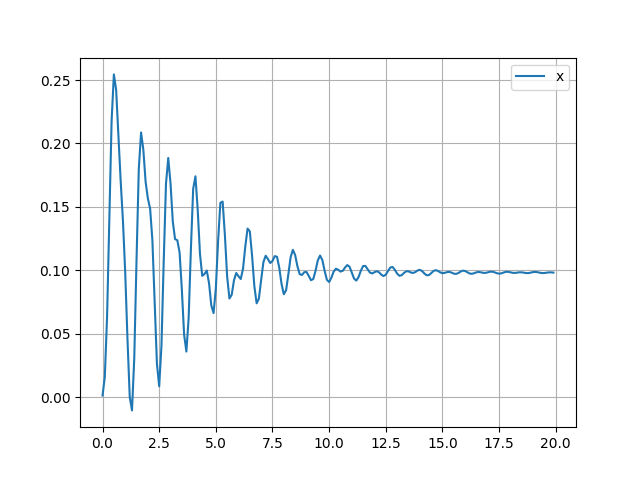
\includegraphics{Appendix/RExpPictures/R/rm1.png}
            \caption{\textit{Case 1 where m = 1 kg}}
            \label{}
        \end{figure}
            
        \begin{figure}[H]
            \centering
            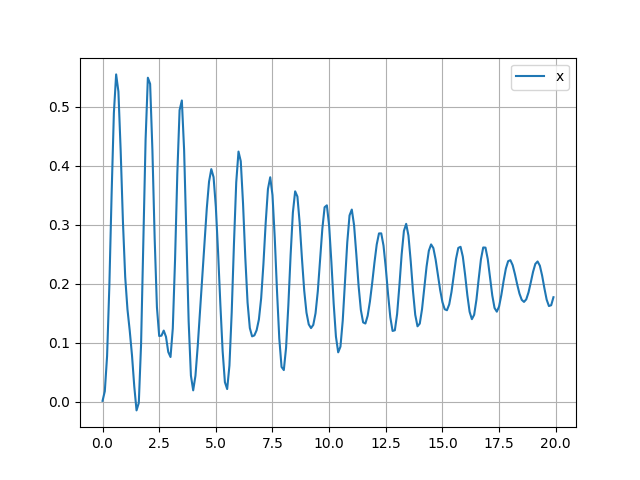
\includegraphics{Appendix/RExpPictures/R/rm2.png}
            \caption{\textit{Case 2 where m = 2 kg}}
            \label{}
        \end{figure}
            
        \begin{figure}[H]
            \centering
            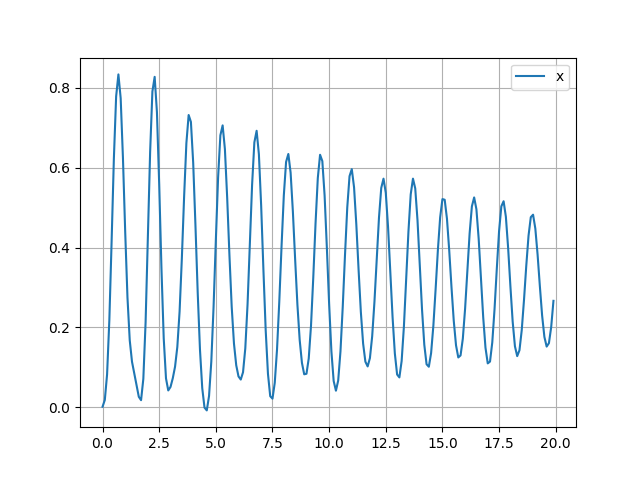
\includegraphics{Appendix/RExpPictures/R/rm3.png}
            \caption{\textit{Case 3 where m = 3 kg}}
            \label{}
        \end{figure}
            
        \begin{figure}[H]
            \centering
            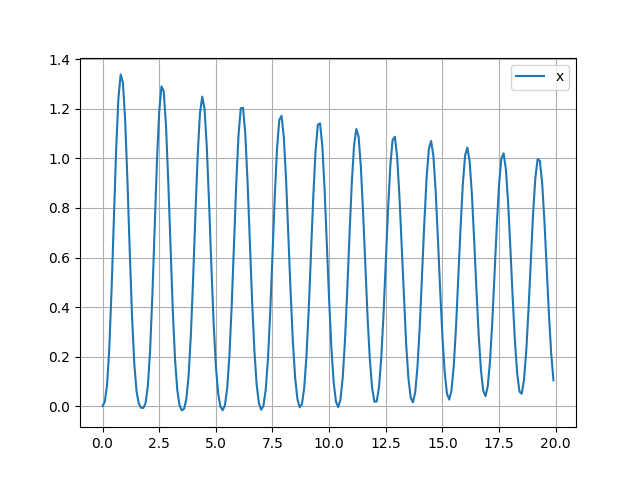
\includegraphics{Appendix/RExpPictures/R/rm5.png}
            \caption{\textit{Case 4 where m = 4 kg}}
            \label{}
        \end{figure}
            
        \begin{figure}[H]
            \centering
            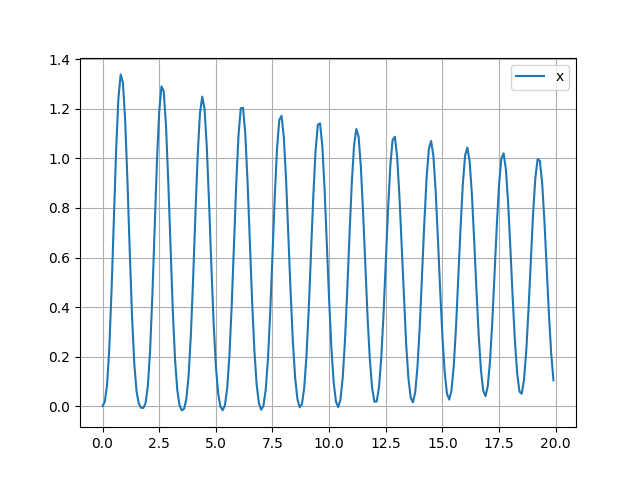
\includegraphics{Appendix/RExpPictures/R/rm5.png}
            \caption{\textit{Case 5 where m = 5 kg}}
            \label{}
        \end{figure}
            
        \begin{figure}[H]
            \centering
            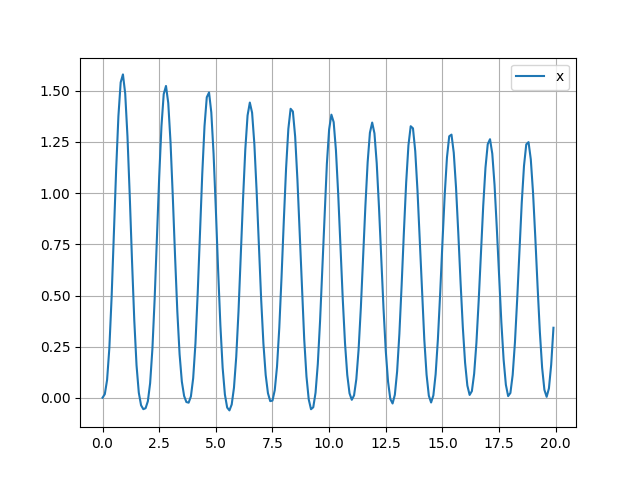
\includegraphics{Appendix/RExpPictures/R/rm6.png}
            \caption{\textit{Case 6 where m = 6 kg}}
            \label{}
        \end{figure}
            
        \begin{figure}[H]
            \centering
            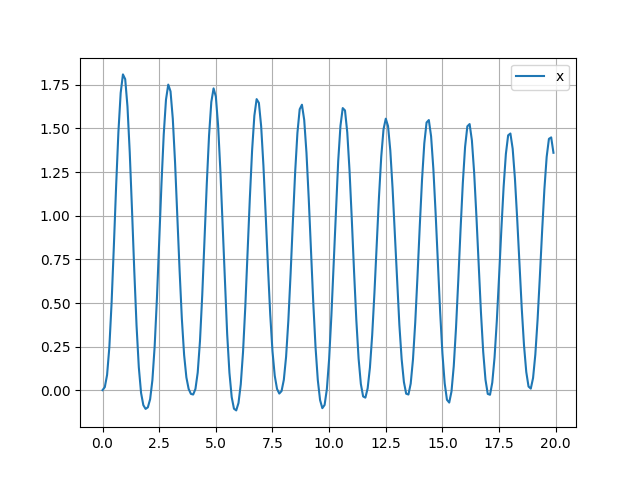
\includegraphics{Appendix/RExpPictures/R/rm7.png}
            \caption{\textit{Case 7 where m = 7 kg}}
            \label{}
        \end{figure}
            
        \begin{figure}[H]
            \centering
            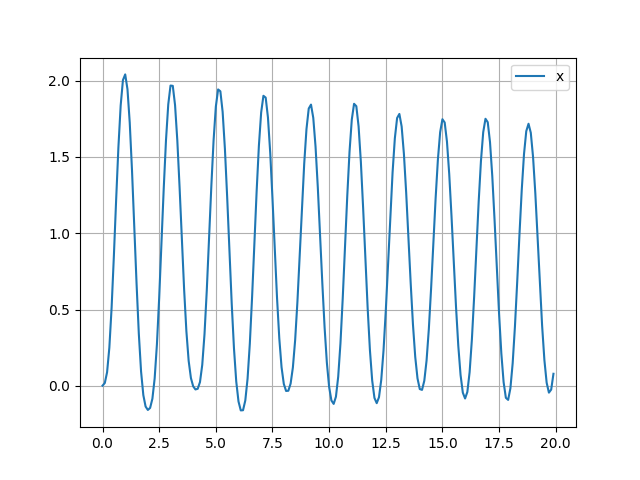
\includegraphics{Appendix/RExpPictures/R/rm8.png}
            \caption{\textit{Case 8 where m = 8 kg}}
            \label{}
        \end{figure}
            
        \begin{figure}[H]
            \centering
            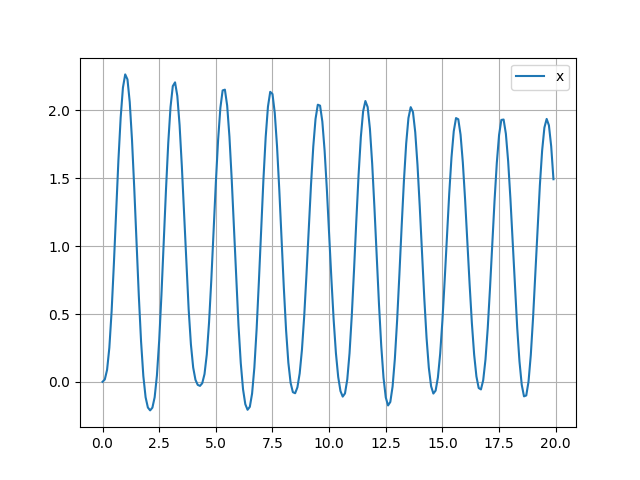
\includegraphics{Appendix/RExpPictures/R/rm9.png}
            \caption{\textit{Case 9 where m = 9 kg}}
            \label{}
        \end{figure}
            
        \begin{figure}[H]
            \centering
            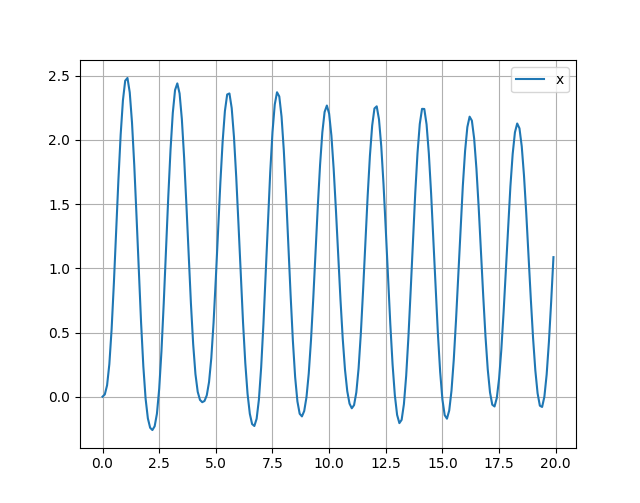
\includegraphics{Appendix/RExpPictures/R/rm10.png}
            \caption{\textit{Case 10 where m = 10 kg}}
            \label{}
        \end{figure}
            
    \section{\textit{Angular Displacement versus Time}}
            
        \begin{figure}[H]
            \centering
            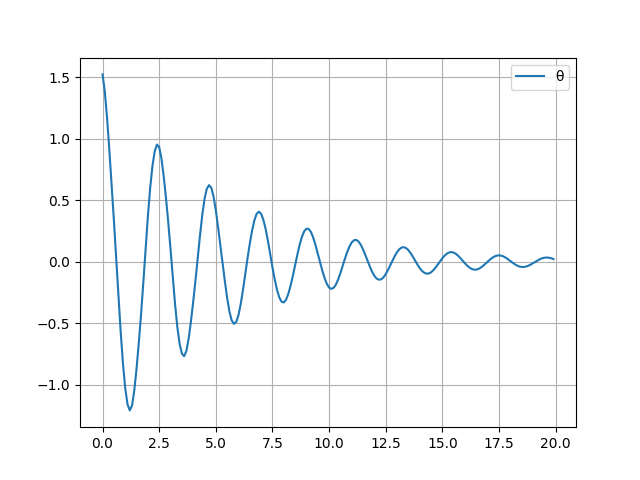
\includegraphics{Appendix/RExpPictures/A/am1.png}
            \caption{\textit{Case 1 where m = 1 kg}}
            \label{}
        \end{figure}
            
        \begin{figure}[H]
            \centering
            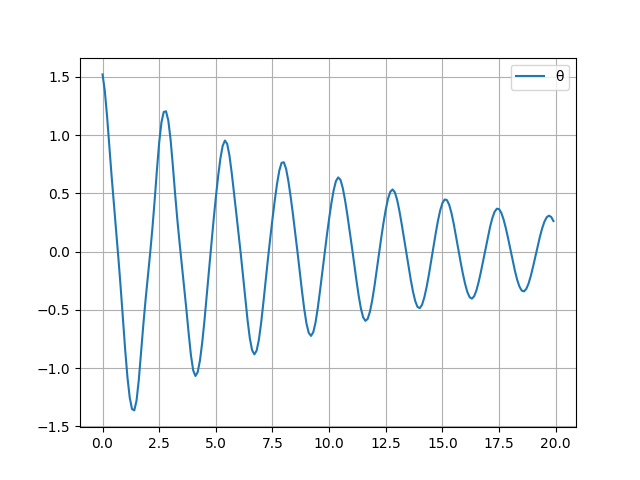
\includegraphics{Appendix/RExpPictures/A/am2.png}
            \caption{\textit{Case 2 where m = 2 kg}}
            \label{}
        \end{figure}
            
        \begin{figure}[H]
            \centering
            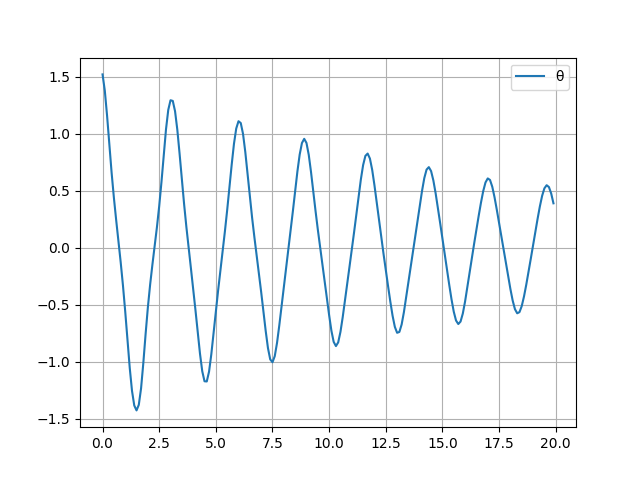
\includegraphics{Appendix/RExpPictures/A/am3.png}
            \caption{\textit{Case 3 where m = 3 kg}}
            \label{}
        \end{figure}
            
        \begin{figure}[H]
            \centering
            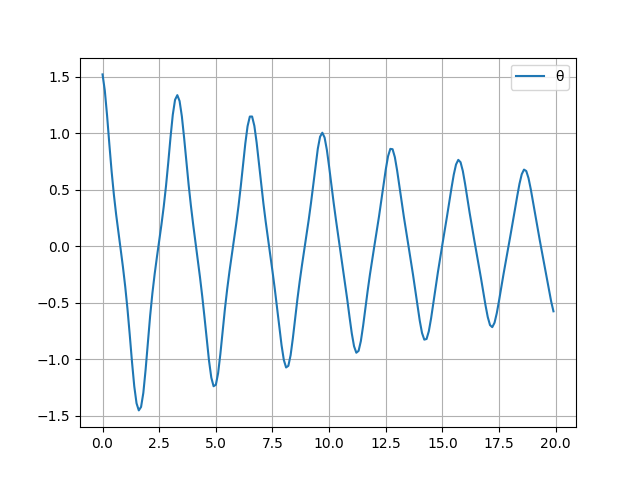
\includegraphics{Appendix/RExpPictures/A/am4.png}
            \caption{\textit{Case 4 where m = 4 kg}}
            \label{}
        \end{figure}
            
        \begin{figure}[H]
            \centering
            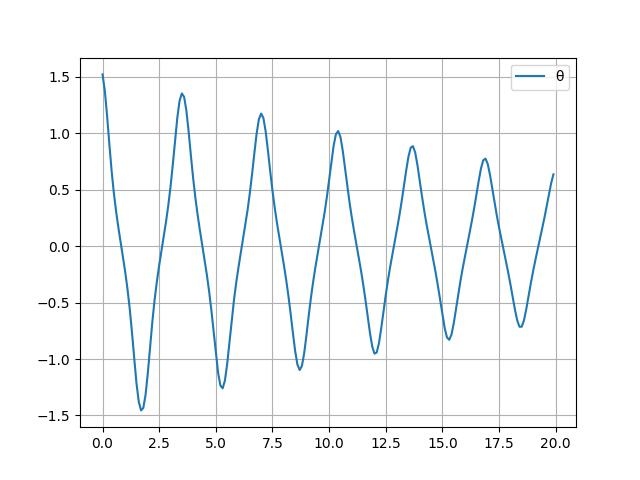
\includegraphics{Appendix/RExpPictures/A/am5.png}
            \caption{\textit{Case 5 where m = 5 kg}}
            \label{}
        \end{figure}
            
        \begin{figure}[H]
            \centering
            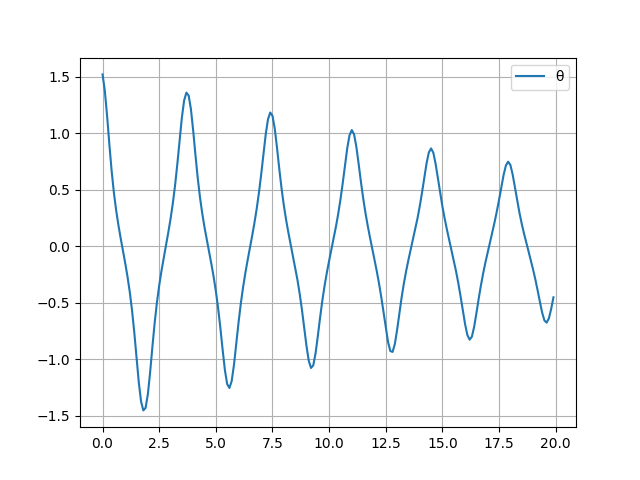
\includegraphics{Appendix/RExpPictures/A/am6.png}
            \caption{\textit{Case 6 where m = 6 kg}}
            \label{}
        \end{figure}
            
        \begin{figure}[H]
            \centering
            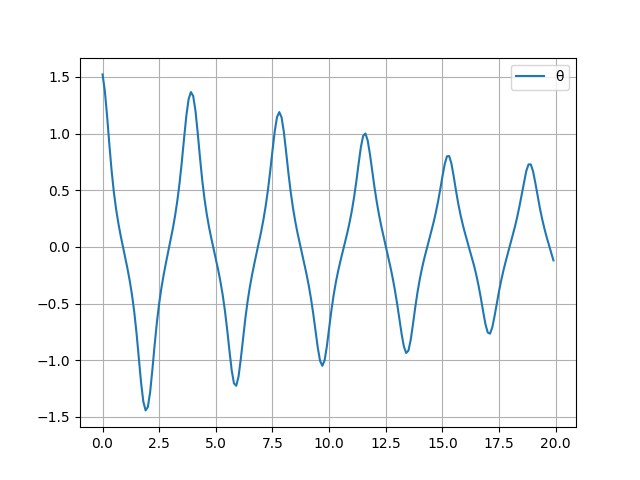
\includegraphics{Appendix/RExpPictures/A/am7.png}
            \caption{\textit{Case 7 where m = 7 kg}}
            \label{}
        \end{figure}
            
        \begin{figure}[H]
            \centering
            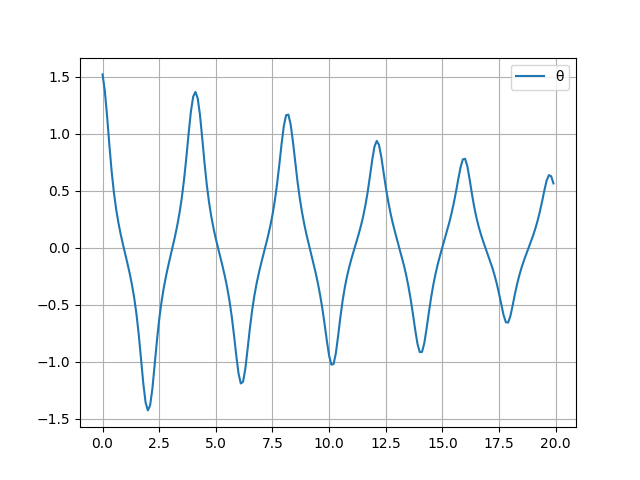
\includegraphics{Appendix/RExpPictures/A/am8.png}
            \caption{\textit{Case 8 where m = 8 kg}}
            \label{}
        \end{figure}
            
        \begin{figure}[H]
            \centering
            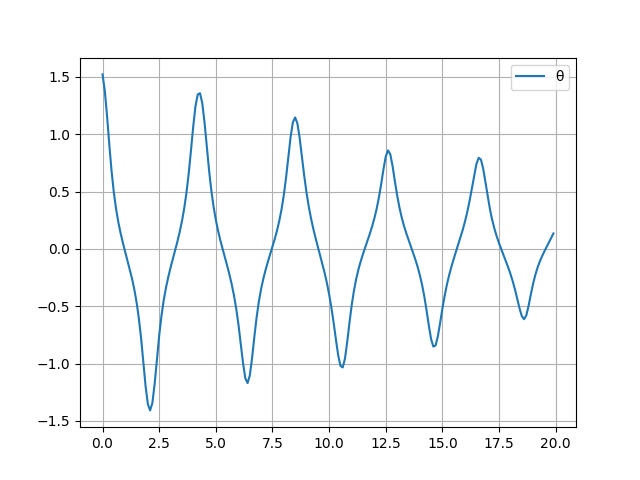
\includegraphics{Appendix/RExpPictures/A/am9.png}
            \caption{\textit{Case 9 where m = 9 kg}}
            \label{}
        \end{figure}
            
        \begin{figure}[H]
            \centering
            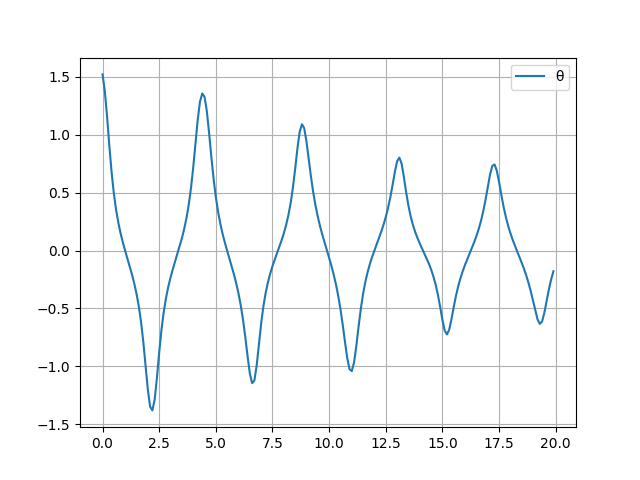
\includegraphics{Appendix/RExpPictures/A/am10.png}
            \caption{\textit{Case 10 where m = 10 kg}}
            \label{}
        \end{figure}
            
    \section{\textit{Angular Frequency versus Time}}
            
        \begin{figure}[H]
            \centering
            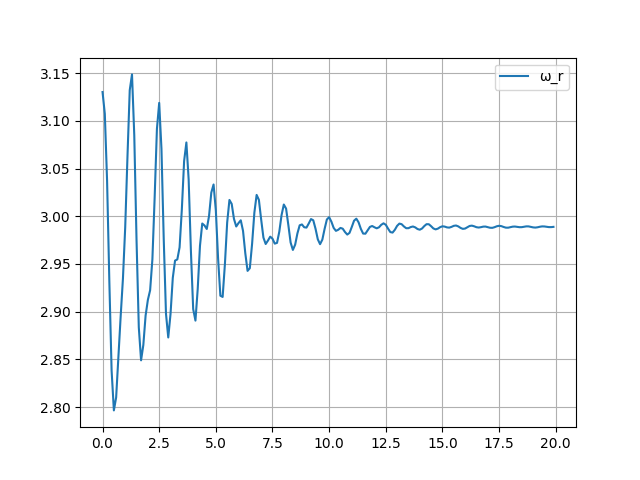
\includegraphics{Appendix/RExpPictures/F/fm1.png}
            \caption{\textit{Case 1 where m = 1 kg}}
            \label{}
        \end{figure}
            
        \begin{figure}[H]
            \centering
            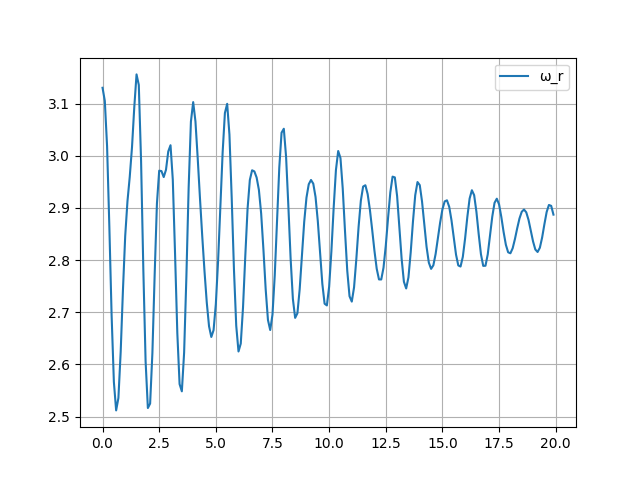
\includegraphics{Appendix/RExpPictures/F/fm2.png}
            \caption{\textit{Case 2 where m = 2 kg}}
            \label{}
        \end{figure}
            
        \begin{figure}[H]
            \centering
            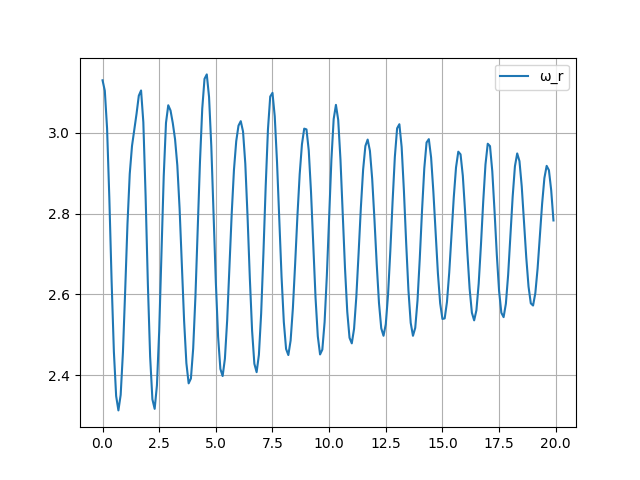
\includegraphics{Appendix/RExpPictures/F/fm3.png}
            \caption{\textit{Case 3 where m = 3 kg}}
            \label{}
        \end{figure}
            
        \begin{figure}[H]
            \centering
            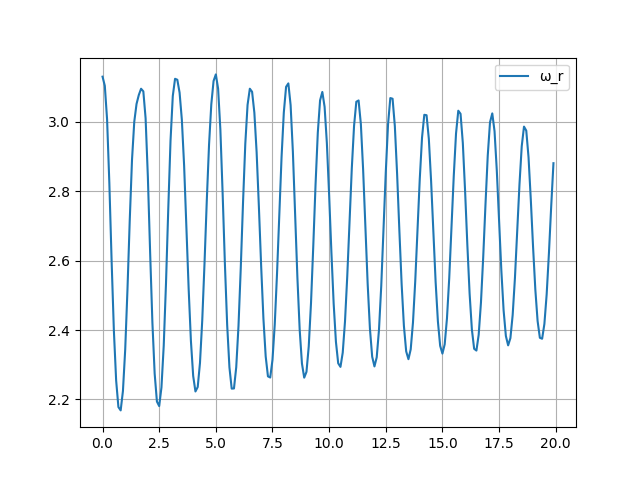
\includegraphics{Appendix/RExpPictures/F/fm4.png}
            \caption{\textit{Case 4 where m = 4 kg}}
            \label{}
        \end{figure}
            
        \begin{figure}[H]
            \centering
            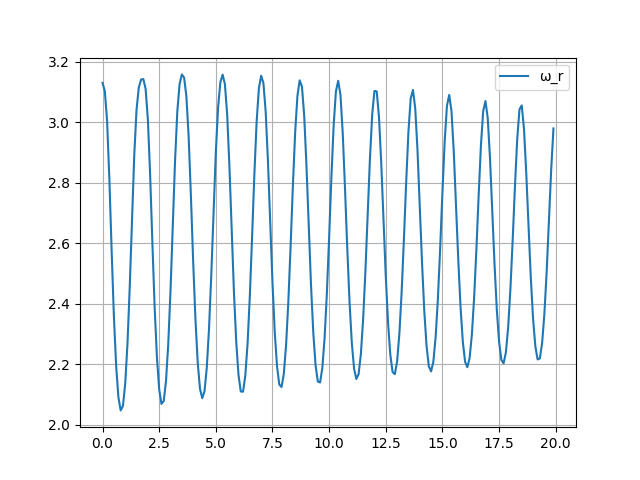
\includegraphics{Appendix/RExpPictures/F/fm5.png}
            \caption{\textit{Case 5 where m = 5 kg}}
            \label{}
        \end{figure}
            
        \begin{figure}[H]
            \centering
            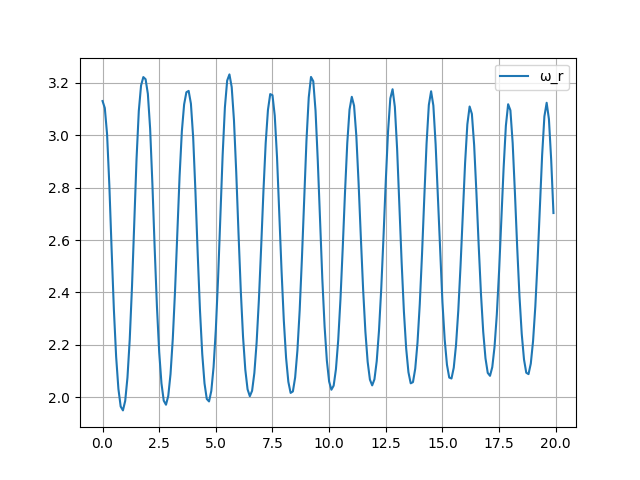
\includegraphics{Appendix/RExpPictures/F/fm6.png}
            \caption{\textit{Case 6 where m = 6 kg}}
            \label{}
        \end{figure}
            
        \begin{figure}[H]
            \centering
            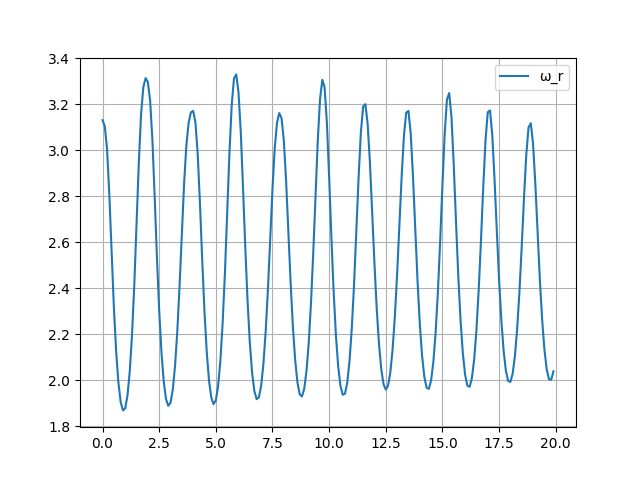
\includegraphics{Appendix/RExpPictures/F/fm7.png}
            \caption{\textit{Case 7 where m = 7 kg}}
            \label{}
        \end{figure}
            
        \begin{figure}[H]
            \centering
            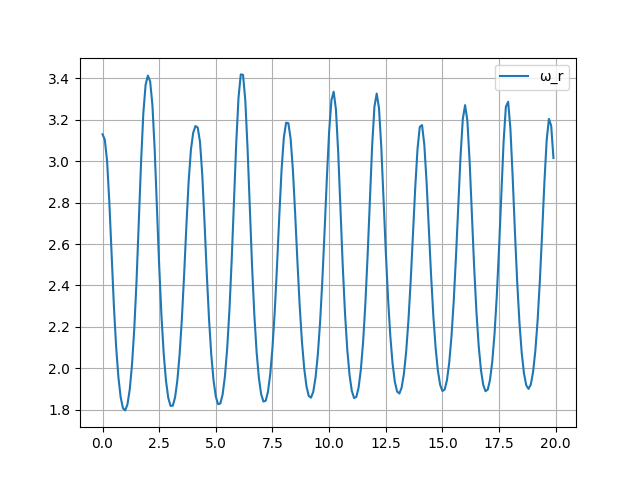
\includegraphics{Appendix/RExpPictures/F/fm8.png}
            \caption{\textit{Case 8 where m = 8 kg}}
            \label{}
        \end{figure}
            
        \begin{figure}[H]
            \centering
            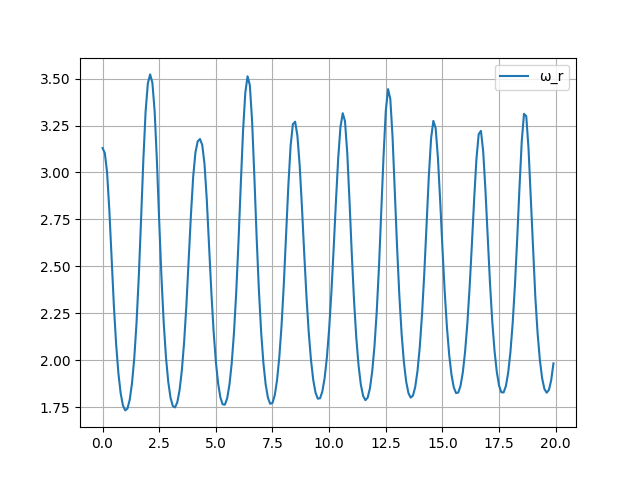
\includegraphics{Appendix/RExpPictures/F/fm9.png}
            \caption{\textit{Case 9 where m = 9 kg}}
            \label{}
        \end{figure}
            
        \begin{figure}[H]
            \centering
            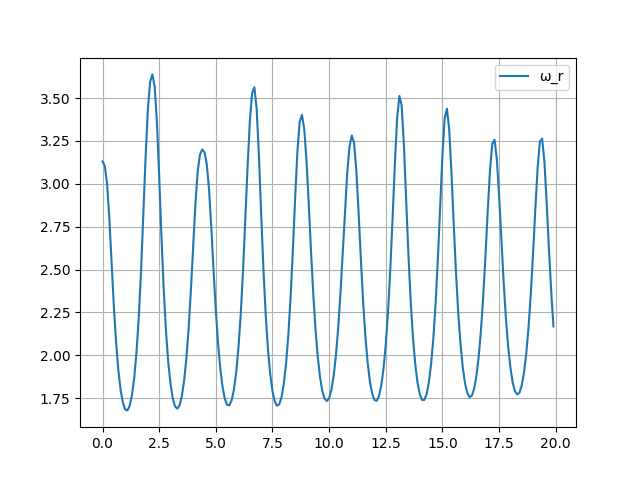
\includegraphics{Appendix/RExpPictures/F/fm10.png}
            \caption{\textit{Case 10 where m = 10 kg}}
            \label{}
        \end{figure}
            
    \section{\textit{Absolute Frequency versus Time}}
            
        \begin{figure}[H]
            \centering
            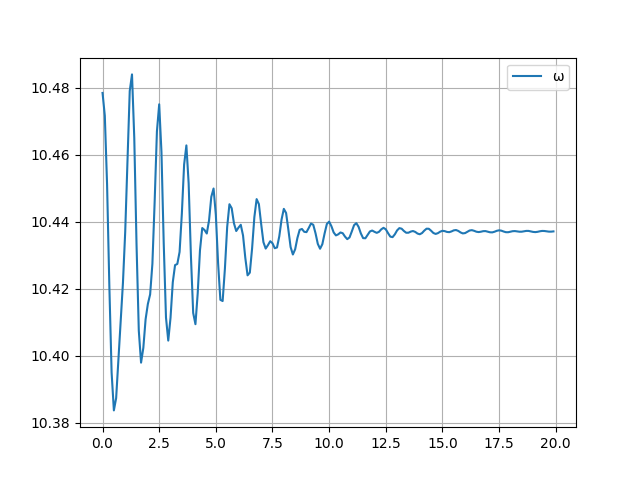
\includegraphics{Appendix/RExpPictures/AF/afm1.png}
            \caption{\textit{Case 1 where m = 1 kg}}
            \label{}
        \end{figure}
            
        \begin{figure}[H]
            \centering
            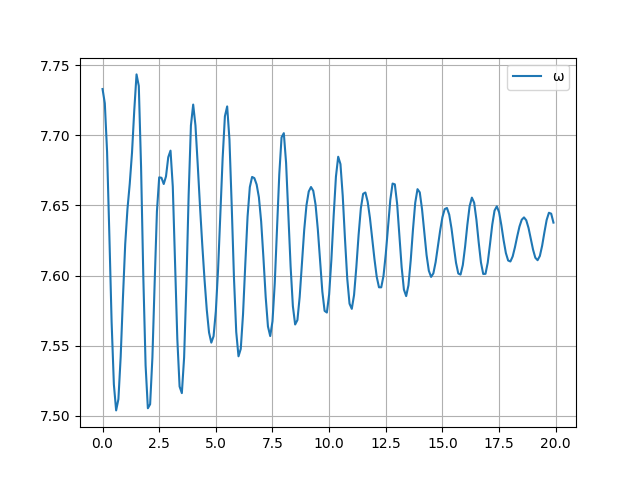
\includegraphics{Appendix/RExpPictures/AF/afm2.png}
            \caption{\textit{Case 2 where m = 2 kg}}
            \label{}
        \end{figure}
            
        \begin{figure}[H]
            \centering
            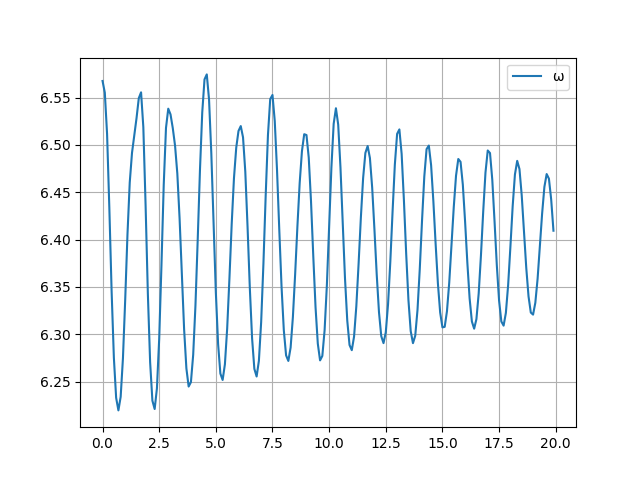
\includegraphics{Appendix/RExpPictures/AF/afm3.png}
            \caption{\textit{Case 3 where m = 3 kg}}
            \label{}
        \end{figure}
            
        \begin{figure}[H]
            \centering
            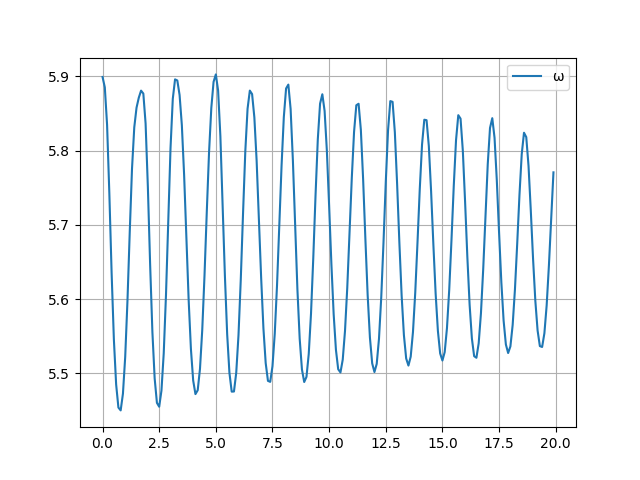
\includegraphics{Appendix/RExpPictures/AF/afm4.png}
            \caption{\textit{Case 4 where m = 4 kg}}
            \label{}
        \end{figure}
            
        \begin{figure}[H]
            \centering
            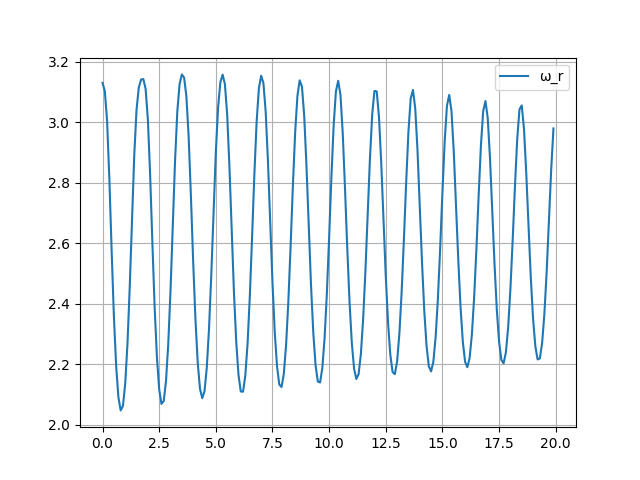
\includegraphics{Appendix/RExpPictures/F/fm5.png}
            \caption{\textit{Case 5 where m = 5 kg}}
            \label{}
        \end{figure}
            
        \begin{figure}[H]
            \centering
            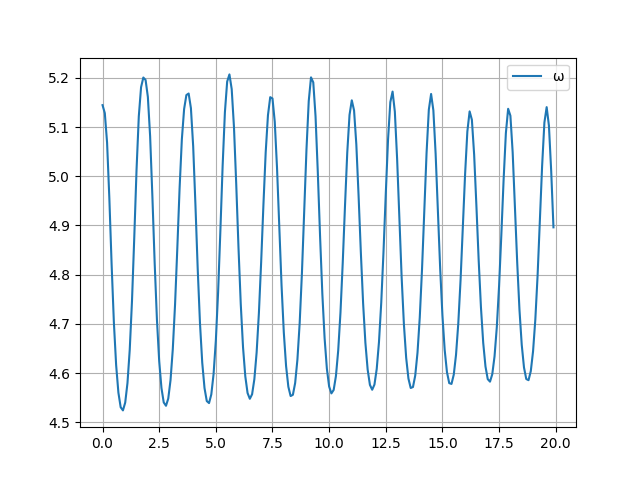
\includegraphics{Appendix/RExpPictures/AF/afm6.png}
            \caption{\textit{Case 6 where m = 6 kg}}
            \label{}
        \end{figure}
            
        \begin{figure}[H]
            \centering
            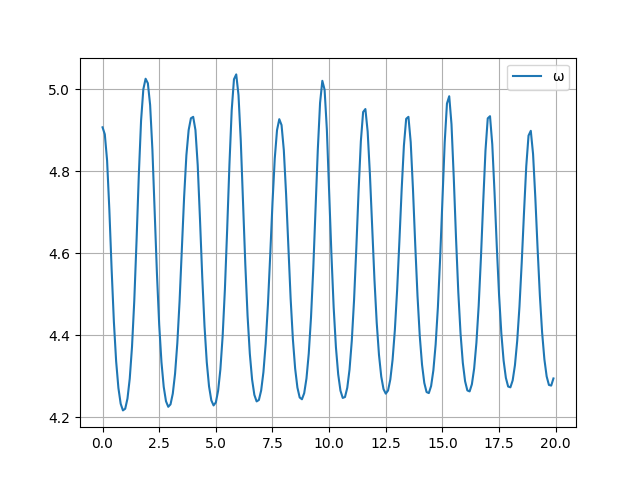
\includegraphics{Appendix/RExpPictures/AF/afm7.png}
            \caption{\textit{Case 7 where m = 7 kg}}
            \label{}
        \end{figure}
            
        \begin{figure}[H]
            \centering
            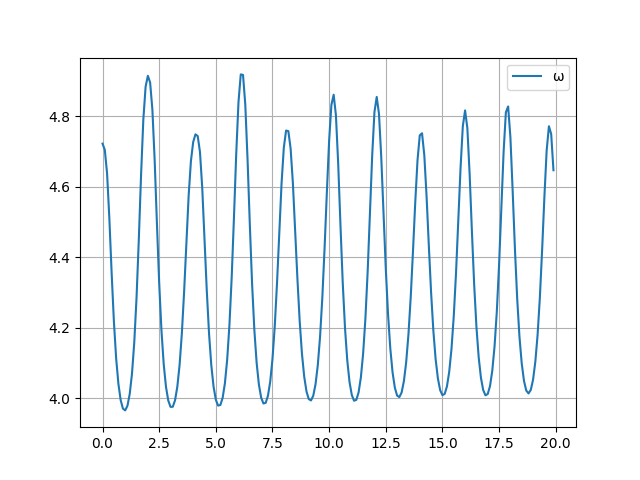
\includegraphics{Appendix/RExpPictures/AF/afm8.png}
            \caption{\textit{Case 8 where m = 8 kg}}
            \label{}
        \end{figure}
            
        \begin{figure}[H]
            \centering
            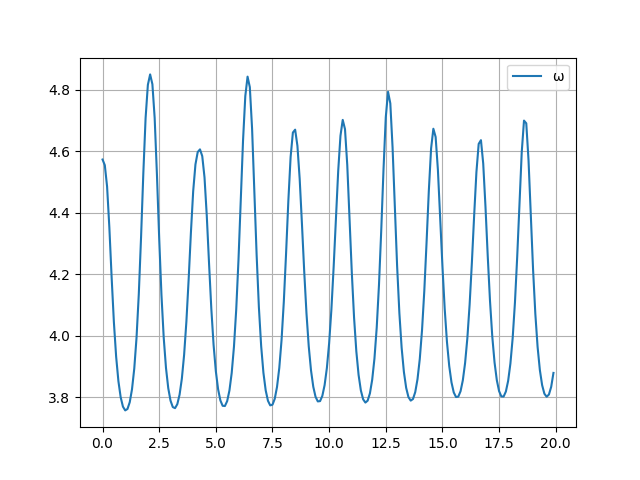
\includegraphics{Appendix/RExpPictures/AF/afm9.png}
            \caption{\textit{Case 9 where m = 9 kg}}
            \label{}
        \end{figure}
            
        \begin{figure}[H]
            \centering
            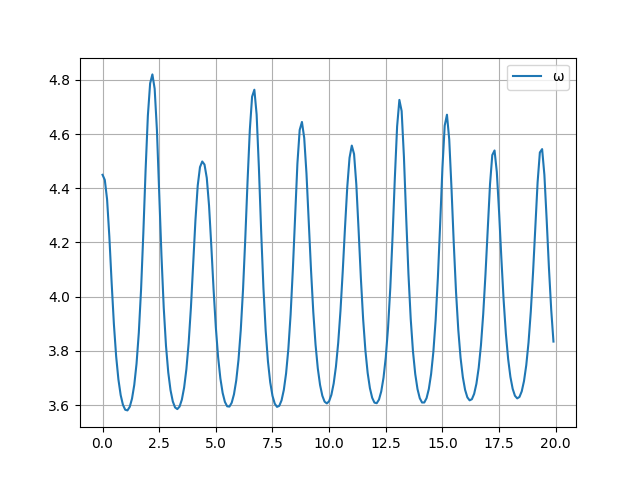
\includegraphics{Appendix/RExpPictures/AF/afm10.png}
            \caption{\textit{Case 10 where m = 10 kg}}
            \label{}
        \end{figure}
            
            
   






